%\part{Einleitung}

\chapter{Programmlogik}
\section{Abschnitt}
\subsection{Teilabschnitt}
\subsubsection{Unterteilabschnitt}
\paragraph{Paragraph}
\subparagraph{Unterparagraph}

\begin{enumerate}
     \item Eine
     \item kleine
     \item Aufzählung
\end{enumerate}

Unter dem Punkt Programmlogik wird der ganze Anfrageprozess verstanden. Dieser beginnt beim Extrahieren von \lstinline|SearchModel|s bis zum Ausliefern der \lstinline|SearchResult|s und wird in folgende Komponenten gegliedert:

\begin{enumerate}
     \item \lstinline|SEARCHExtraction|
     \item \lstinline|QueryCreation|
     \item \lstinline|QueryResolution|
     \item \lstinline|Ranking|
\end{enumerate}

\begin{figure}[htb]
  \centering
  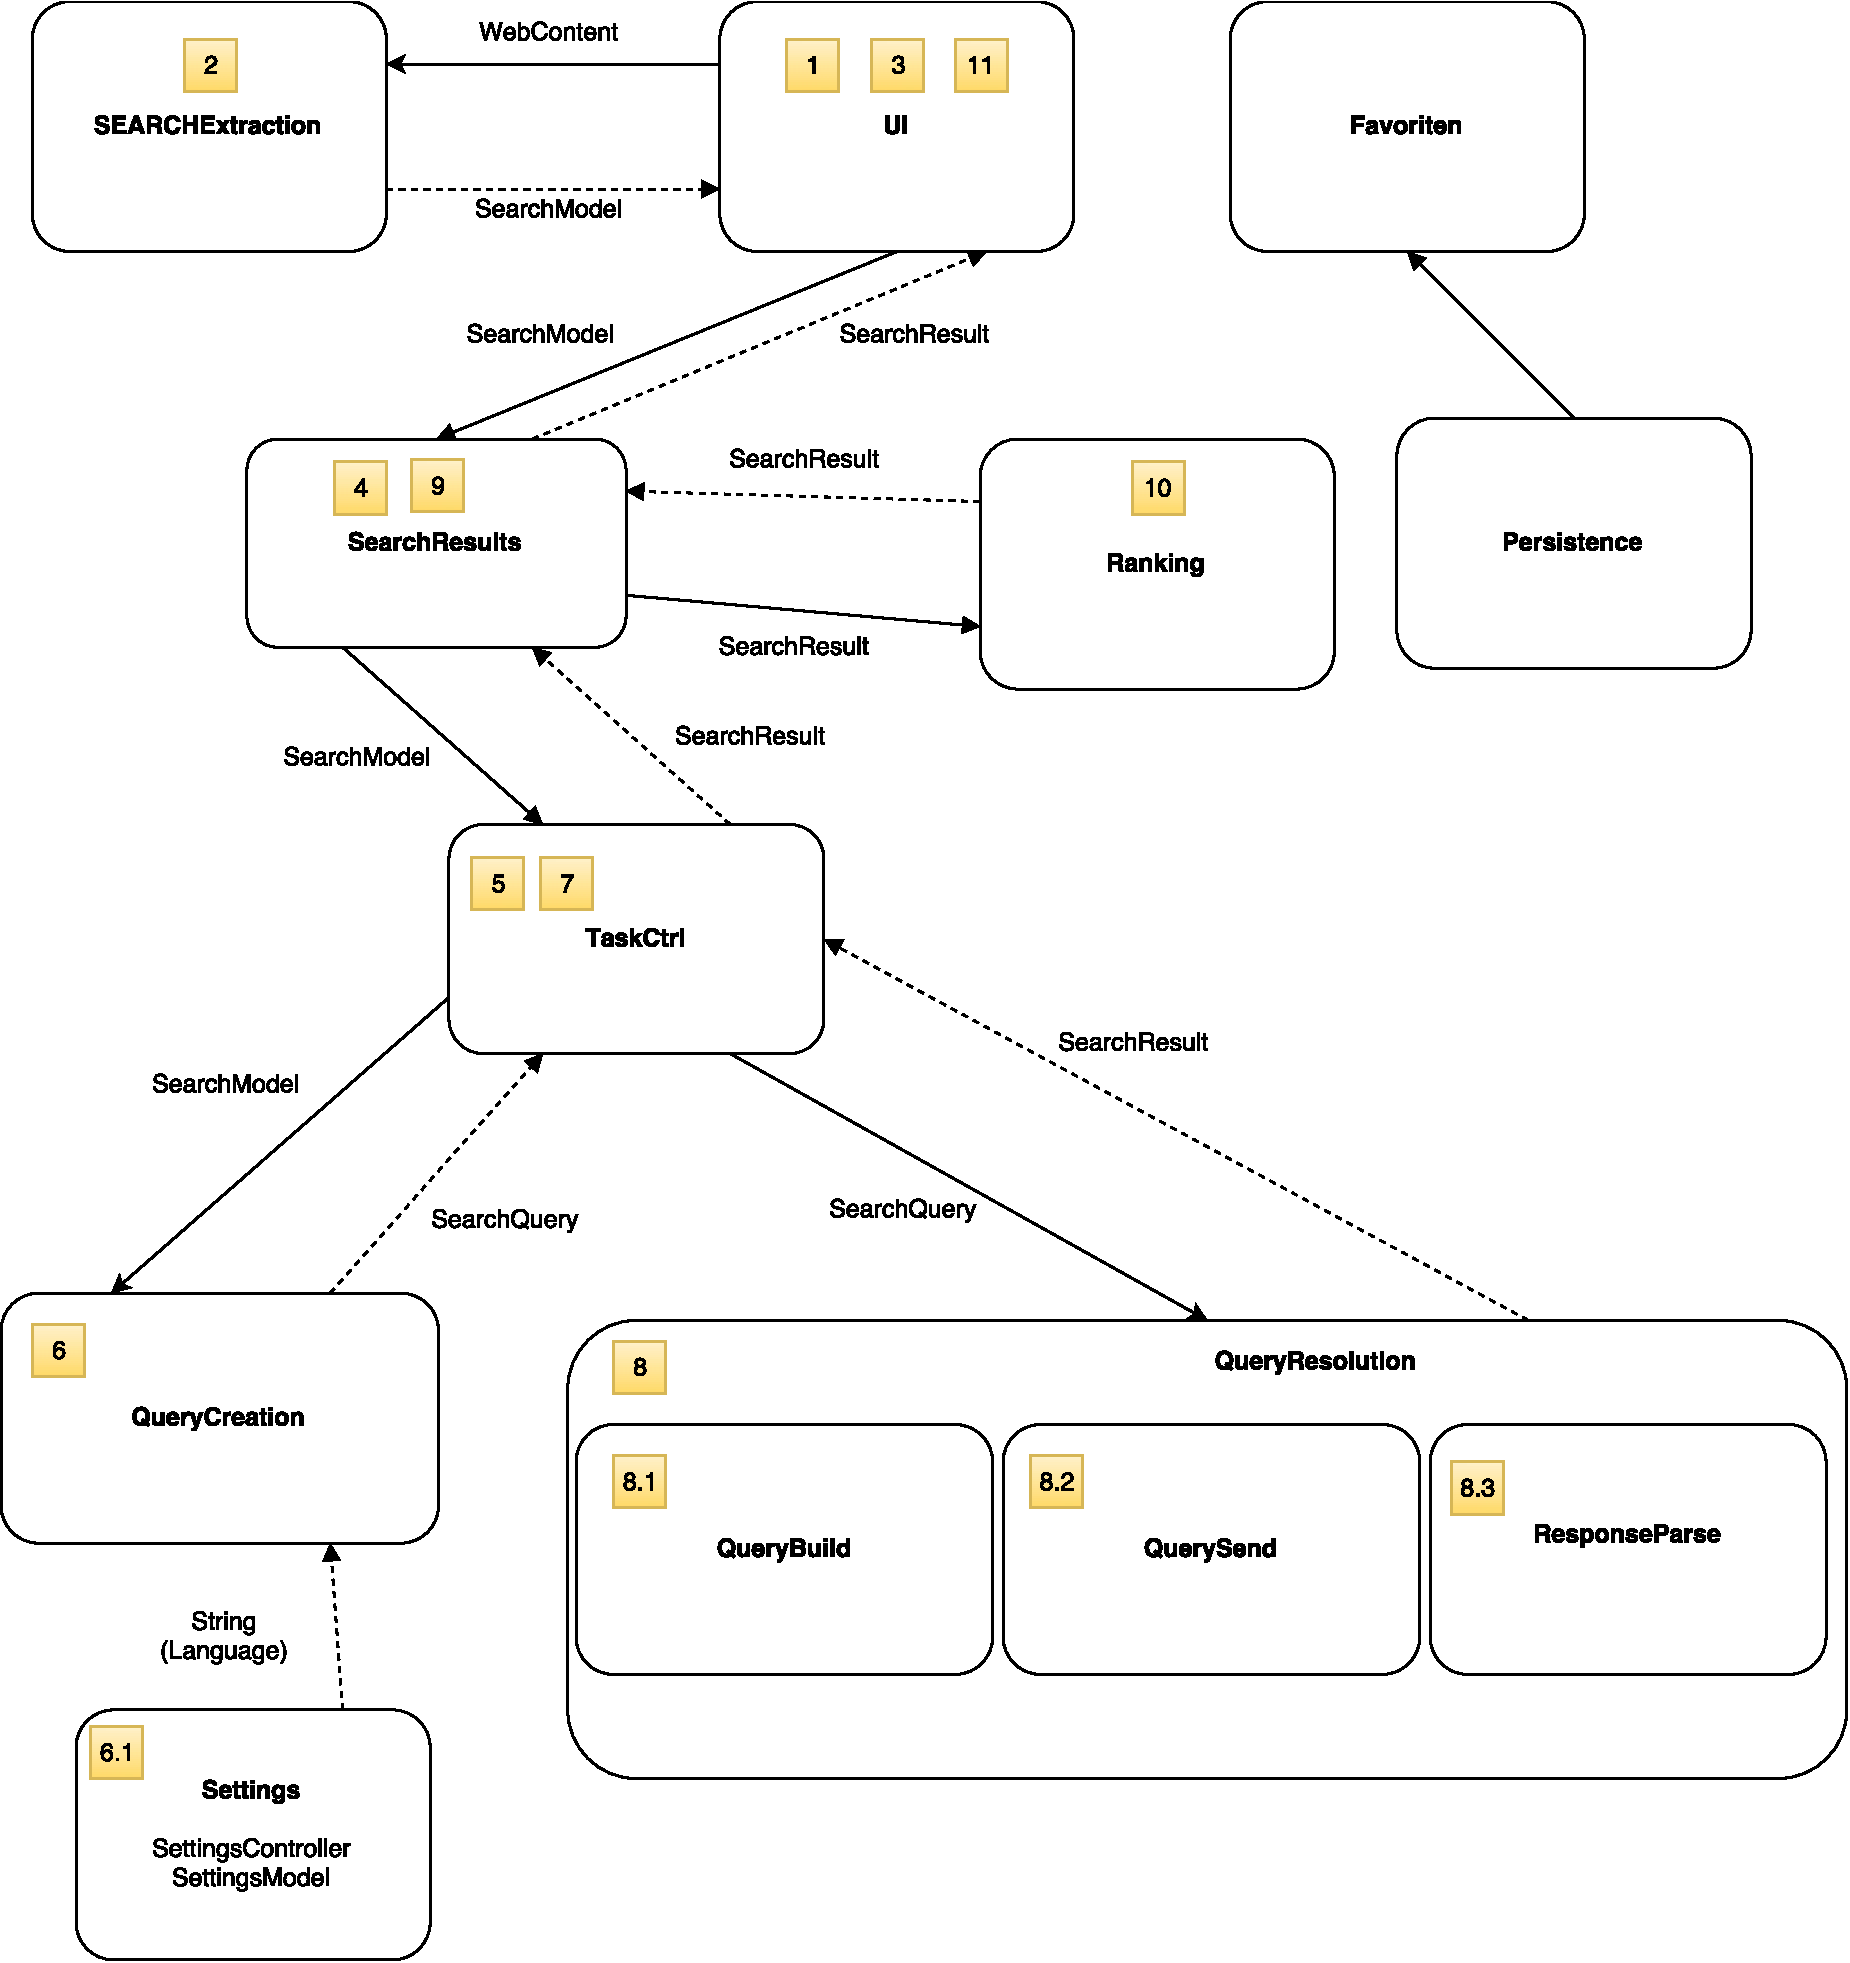
\includegraphics[width=0.6\textwidth]{Architektur}
  \caption{Übersicht des Kapitels Programmlogik}
\end{figure}

